\section{Results}\label{sec:results}
% Generated by analysis.extended_report from measured extended results; do not edit.
\providecommand{\ExtOneRawAggregationMin}{2.4}
\providecommand{\ExtOneRawAggregationMax}{55.4}
\providecommand{\ExtOneRawRegenerationMin}{-6.1}
\providecommand{\ExtOneRawRegenerationMax}{24.2}
\providecommand{\ExtOneRawTotalMin}{-1.7}
\providecommand{\ExtOneRawTotalMax}{79.6}
\providecommand{\ExtOneRawAggregationPositive}{5}
\providecommand{\ExtOneGzipAggregationMin}{3.3}
\providecommand{\ExtOneGzipAggregationMax}{65.4}
\providecommand{\ExtOneGzipRegenerationMin}{-6.6}
\providecommand{\ExtOneGzipRegenerationMax}{7.0}
\providecommand{\ExtOneGzipTotalMin}{-2.2}
\providecommand{\ExtOneGzipTotalMax}{72.5}
\providecommand{\ExtOneGzipAggregationPositive}{5}
\providecommand{\ExtTwoRawAggregationMin}{2.2}
\providecommand{\ExtTwoRawAggregationMax}{52.8}
\providecommand{\ExtTwoRawRegenerationMin}{-6.2}
\providecommand{\ExtTwoRawRegenerationMax}{23.7}
\providecommand{\ExtTwoRawTotalMin}{-2.5}
\providecommand{\ExtTwoRawTotalMax}{76.5}
\providecommand{\ExtTwoRawAggregationPositive}{5}
\providecommand{\ExtTwoGzipAggregationMin}{3.7}
\providecommand{\ExtTwoGzipAggregationMax}{66.4}
\providecommand{\ExtTwoGzipRegenerationMin}{-6.7}
\providecommand{\ExtTwoGzipRegenerationMax}{5.9}
\providecommand{\ExtTwoGzipTotalMin}{-2.3}
\providecommand{\ExtTwoGzipTotalMax}{72.4}
\providecommand{\ExtTwoGzipAggregationPositive}{5}
\providecommand{\ExtTiles}{45{,}689}
\providecommand{\ExtCheckedAddresses}{91{,}378}
\providecommand{\ExtRoundtripDifferences}{0}
\providecommand{\ExtAggregateBlocks}{9{,}042}

\subsection{Fixed-content aggregation}\label{sec:results-granularity}
All \ExtAggregateBlocks{} aggregate blocks pass the typed feature-multiset check.
The expanded corpus contains \ExtTiles{} MVT addresses, each also encoded as MLT
v1 and v2. Table~\ref{tab:main} reports MLT saving relative to its own MVT input.
For $4\times4$ controlled aggregation, raw v1 byte reductions range from
\ExtOneRawAggregationMin\% to \ExtOneRawAggregationMax\%, positive in
\ExtOneRawAggregationPositive{} datasets; v2 ranges from \ExtTwoRawAggregationMin\%
to \ExtTwoRawAggregationMax\%, positive in \ExtTwoRawAggregationPositive{} datasets.
After gzip the ranges are \ExtOneGzipAggregationMin--\ExtOneGzipAggregationMax\%
and \ExtTwoGzipAggregationMin--\ExtTwoGzipAggregationMax\%. All buffered and clipped
Standard instances are retained in these comparisons.

\begin{table*}[!tp]\centering\small
\caption{MLT savings relative to MVT (\%) within each variant, using byte sums
over addresses. A4/A16 are Aggregated; D4/D16 are Dense.}\label{tab:main}
\begin{tabular}{@{}llrrrrr@{}}\toprule
Dataset & Variant & Tiles & Raw v1 & Raw v2 & Gzip v1 & Gzip v2\\
\midrule% Generated by analysis.extended_report from measured extended results; do not edit.
Natural Earth & Std & 25{,}800 & 34.4 & 52.3 & 10.8 & 14.3 \\
 & A4 & 6{,}554 & 52.8 & 64.9 & 12.4 & 15.9 \\
 & A16 & 1{,}705 & 61.0 & 69.9 & 14.5 & 20.3 \\
 & D4 & 6{,}554 & 38.0 & 52.1 & 14.7 & 17.6 \\
 & D16 & 1{,}705 & 44.5 & 53.4 & 20.0 & 22.9 \\
PDOK BGT & Std & 153 & 62.4 & 63.9 & 28.4 & 29.8 \\
 & A4 & 68 & 62.7 & 64.2 & 29.0 & 30.7 \\
 & A16 & 37 & 63.0 & 64.5 & 29.4 & 31.1 \\
 & D4 & 70 & 62.4 & 64.0 & 29.0 & 30.5 \\
 & D16 & 39 & 62.7 & 64.1 & 29.3 & 30.9 \\
USFWS & Std & 606 & 45.0 & 46.1 & 14.9 & 16.0 \\
 & A4 & 184 & 45.6 & 46.4 & 15.2 & 16.4 \\
 & A16 & 71 & 46.1 & 46.8 & 15.6 & 16.8 \\
 & D4 & 190 & 46.4 & 47.1 & 15.5 & 16.6 \\
 & D16 & 81 & 47.4 & 48.0 & 16.2 & 17.3 \\
swisstopo & Std & 435 & 19.7 & 29.5 & 12.8 & 10.8 \\
 & A4 & 128 & 29.4 & 35.2 & 17.0 & 16.2 \\
 & A16 & 47 & 34.5 & 37.7 & 19.0 & 19.2 \\
 & D4 & 130 & 26.6 & 32.7 & 16.1 & 15.3 \\
 & D16 & 50 & 30.3 & 33.8 & 17.8 & 17.8 \\
OSM & Std & 576 & 46.9 & 53.7 & 13.1 & 17.6 \\
 & A4 & 178 & 48.7 & 54.8 & 14.0 & 19.3 \\
 & A16 & 70 & 49.7 & 55.6 & 14.7 & 20.4 \\
 & D4 & 182 & 49.6 & 55.4 & 14.9 & 20.0 \\
 & D16 & 76 & 50.6 & 56.2 & 16.0 & 21.2 \\
\bottomrule
\end{tabular}\end{table*}
% Generated from docs/data/extended/results.sqlite by analysis.extended_report.
\begin{figure*}[!tp]
\centering
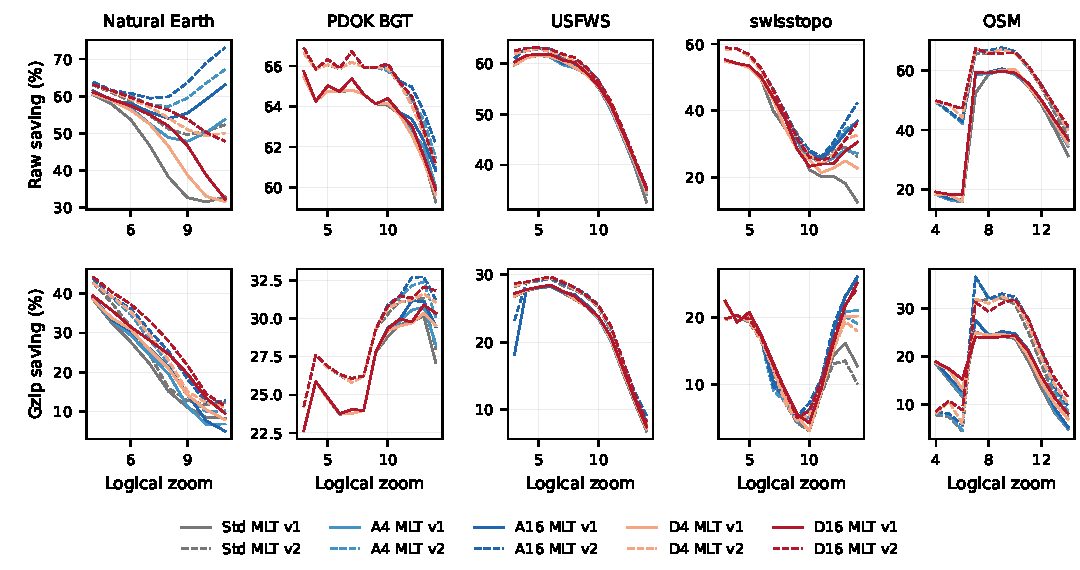
\includegraphics[width=\textwidth]{figures/analysis_zoom_aligned.pdf}
\caption{MLT saving relative to each variant's MVT input by logical zoom,
raw (top) and after independent gzip-6 (bottom). Colours distinguish Standard,
Aggregated-4/16 and Dense-4/16; solid curves are v1 and dashed curves v2.
The additive decomposition separately matches geographic parent blocks.}
\label{fig:zoom-aligned}
\end{figure*}


\subsection{Additional regeneration effects}\label{sec:results-density}
Table~\ref{tab:decomposition} separates aggregation from regeneration. Both components
divide by matched Standard bytes, so they sum to the total reduction. Negative
regeneration values mean that Dense requires more bytes than the exact aggregate.
For $4\times4$ blocks the total gzip reduction ranges from
\ExtOneGzipTotalMin\% to \ExtOneGzipTotalMax\% for v1 and
\ExtTwoGzipTotalMin\% to \ExtTwoGzipTotalMax\% for v2.

\begin{table*}[!tp]\centering\footnotesize
\caption{Additive reductions relative to matched Standard bytes (\%). A: aggregation;
R: regeneration; T: total. Integer bytes and per-zoom values are exported separately;
rounding can change the displayed component sum by 0.1 percentage points.}
\label{tab:decomposition}
\begin{tabular}{@{}lrlrrrrrr@{}}\toprule
& & & \multicolumn{3}{c}{MLT v1} & \multicolumn{3}{c}{MLT v2}\\
Dataset & Factor & State & A & R & T & A & R & T\\
\midrule% Generated by analysis.extended_report from measured extended results; do not edit.
Natural Earth & 4 & raw & 42.1 & 19.4 & 61.5 & 41.0 & 18.1 & 59.1 \\
 & 4 & gzip & 50.7 & 5.0 & 55.8 & 50.8 & 4.8 & 55.5 \\
 & 16 & raw & 55.4 & 24.2 & 79.6 & 52.8 & 23.7 & 76.5 \\
 & 16 & gzip & 65.4 & 7.0 & 72.5 & 66.4 & 5.9 & 72.4 \\
PDOK BGT & 4 & raw & 2.0 & 0.1 & 2.1 & 1.8 & 0.2 & 1.9 \\
 & 4 & gzip & 2.5 & -0.6 & 2.0 & 3.0 & -0.8 & 2.2 \\
 & 16 & raw & 2.4 & 0.9 & 3.3 & 2.2 & 0.8 & 3.0 \\
 & 16 & gzip & 3.3 & -0.2 & 3.0 & 3.7 & -0.4 & 3.3 \\
USFWS & 4 & raw & 3.2 & -2.4 & 0.8 & 2.7 & -2.5 & 0.2 \\
 & 4 & gzip & 2.9 & -2.7 & 0.2 & 3.1 & -2.9 & 0.2 \\
 & 16 & raw & 4.4 & -6.1 & -1.7 & 3.7 & -6.2 & -2.5 \\
 & 16 & gzip & 4.3 & -6.6 & -2.2 & 4.4 & -6.7 & -2.3 \\
swisstopo & 4 & raw & 31.2 & 2.5 & 33.7 & 28.1 & 2.6 & 30.7 \\
 & 4 & gzip & 25.9 & 2.6 & 28.5 & 26.8 & 2.6 & 29.4 \\
 & 16 & raw & 42.1 & 4.2 & 46.3 & 37.3 & 4.5 & 41.7 \\
 & 16 & gzip & 34.4 & 4.5 & 38.9 & 36.0 & 4.3 & 40.3 \\
OSM & 4 & raw & 7.5 & -1.6 & 5.8 & 6.4 & -2.0 & 4.4 \\
 & 4 & gzip & 6.1 & -1.3 & 4.8 & 7.0 & -1.6 & 5.5 \\
 & 16 & raw & 10.2 & -5.6 & 4.5 & 8.9 & -6.0 & 2.9 \\
 & 16 & gzip & 8.3 & -4.4 & 3.9 & 9.6 & -4.8 & 4.8 \\
\bottomrule
\end{tabular}\end{table*}

Standard and Aggregated feature and vertex totals are exactly equal over matched
blocks; Dense need not preserve them (Table~\ref{tab:content-differences}). Components
include inherent multipart geometry and rings. Repeated coordinates identify
observable ID/coordinate redundancy within a block, without attributing its cause.

\begin{table*}[!tp]\centering\footnotesize
\caption{Matched content counts (thousands). A: Aggregated; D: Dense. Repeated vertices
share ID and coordinates within a block.}\label{tab:content-differences}
\setlength{\tabcolsep}{3pt}
\begin{tabular}{@{}lrrrrrrrrr@{}}\toprule
& & \multicolumn{2}{c}{Instances} & \multicolumn{2}{c}{Vertices} &
\multicolumn{2}{c}{Source IDs$^*$} & \multicolumn{2}{c}{Repeated vertices}\\
Dataset & Factor & A & D & A & D & A & D & A & D\\
\midrule% Generated by analysis.extended_report from measured extended results; do not edit.
Natural Earth & 4 & 1{,}982.7 & 978.3 & 17{,}994.6 & 14{,}127.0 & 473.8 & 473.8 & 435.0 & 30.5 \\
 & 16 & 1{,}982.7 & 683.4 & 17{,}994.6 & 13{,}028.3 & 473.8 & 473.8 & 651.5 & 31.0 \\
PDOK BGT & 4 & 1{,}124.0 & 1{,}101.1 & 10{,}342.3 & 10{,}156.2 & 1{,}079.2 & 1{,}079.2 & 448.3 & 174.7 \\
 & 16 & 1{,}124.0 & 1{,}087.5 & 10{,}342.3 & 10{,}015.8 & 1{,}079.2 & 1{,}079.1 & 531.4 & 173.3 \\
USFWS & 4 & 333.8 & 343.3 & 13{,}807.2 & 13{,}930.4 & 279.5 & 279.4 & 548.1 & 94.2 \\
 & 16 & 333.8 & 361.6 & 13{,}807.2 & 14{,}226.0 & 279.5 & 279.4 & 763.7 & 103.3 \\
swisstopo & 4 & 4.6 & 3.3 & 174.4 & 168.0 & 2.4 & 2.4 & 5.6 & 0.2 \\
 & 16 & 4.6 & 2.8 & 174.4 & 163.3 & 2.4 & 2.4 & 8.2 & 0.2 \\
OSM & 4 & 123.0 & 123.7 & 2{,}048.6 & 2{,}077.7 & 102.2 & 102.2 & 79.0 & 9.1 \\
 & 16 & 123.0 & 127.9 & 2{,}048.6 & 2{,}147.2 & 102.2 & 102.2 & 112.5 & 9.9 \\
\bottomrule
\end{tabular}
\par\smallskip $^*$Unique IDs at each logical zoom, summed across zooms.
\end{table*}

\subsection{Robustness across MLT versions}\label{sec:results-versions}
The paired version comparison holds MVT input and shared encoder settings fixed.
Tables~\ref{tab:main} and~\ref{tab:decomposition} show both the version-specific
relative saving and the controlled aggregation component. Figure~\ref{fig:zoom-aligned}
shows individual logical zooms; absolute totals are dominated by the zooms carrying
most bytes. The decomposition uses common parent blocks, while a coverage export
records unmatched edge support.

\subsection{Stream structure}\label{sec:results-streams}
The native walker accounts for all bytes in every converted MLT tile. Structural
share, expanded logical values per stream and payload bytes per logical value use
consistent definitions in both versions (Table~\ref{tab:streams}). Stream-role
mixtures can change with regeneration; Aggregated provides the stronger control.
These descriptive measurements do not individually establish a causal contribution
to after-gzip savings.

\begin{table*}[!tp]\centering\footnotesize
\caption{Stream structure per unique MVT payload input, using expanded integer-RLE
counts. Structural share is $(F-P)/F$.}\label{tab:streams}
\begin{tabular}{@{}llrrrrrr@{}}\toprule
& & \multicolumn{2}{c}{Values/stream} & \multicolumn{2}{c}{Structure (\%)} & \multicolumn{2}{c}{Payload B/value}\\
Dataset & Variant & v1 & v2 & v1 & v2 & v1 & v2\\
\midrule% Generated by analysis.extended_report from measured extended results; do not edit.
Natural Earth & Std & 34 & 27 & 40.61 & 34.76 & 0.403 & 0.610 \\
 & A4 & 111 & 79 & 22.37 & 17.59 & 0.305 & 0.514 \\
 & A16 & 362 & 249 & 9.03 & 6.83 & 0.273 & 0.472 \\
 & D4 & 47 & 38 & 31.59 & 25.38 & 0.431 & 0.682 \\
 & D16 & 92 & 75 & 18.64 & 13.67 & 0.440 & 0.732 \\
PDOK BGT & Std & 2{,}254 & 3{,}375 & 0.46 & 0.36 & 1.239 & 0.786 \\
 & A4 & 4{,}429 & 6{,}589 & 0.24 & 0.19 & 1.220 & 0.777 \\
 & A16 & 6{,}641 & 9{,}787 & 0.16 & 0.12 & 1.218 & 0.779 \\
 & D4 & 4{,}225 & 6{,}292 & 0.25 & 0.19 & 1.238 & 0.789 \\
 & D16 & 6{,}080 & 9{,}056 & 0.17 & 0.13 & 1.239 & 0.791 \\
USFWS & Std & 668 & 933 & 0.98 & 0.65 & 1.331 & 1.227 \\
 & A4 & 1{,}901 & 2{,}557 & 0.35 & 0.23 & 1.303 & 1.228 \\
 & A16 & 5{,}013 & 6{,}654 & 0.14 & 0.09 & 1.275 & 1.225 \\
 & D4 & 2{,}028 & 2{,}814 & 0.33 & 0.22 & 1.320 & 1.234 \\
 & D16 & 4{,}856 & 6{,}672 & 0.14 & 0.09 & 1.316 & 1.235 \\
swisstopo & Std & 38 & 62 & 10.24 & 8.77 & 2.157 & 1.138 \\
 & A4 & 119 & 145 & 4.81 & 3.89 & 1.597 & 1.154 \\
 & A16 & 313 & 338 & 2.25 & 1.71 & 1.397 & 1.176 \\
 & D4 & 107 & 136 & 5.00 & 4.08 & 1.709 & 1.172 \\
 & D16 & 257 & 292 & 2.48 & 1.92 & 1.512 & 1.204 \\
OSM & Std & 272 & 330 & 2.51 & 1.86 & 1.147 & 0.813 \\
 & A4 & 666 & 770 & 1.15 & 0.81 & 1.052 & 0.786 \\
 & A16 & 1{,}376 & 1{,}550 & 0.61 & 0.42 & 1.010 & 0.770 \\
 & D4 & 683 & 787 & 1.13 & 0.80 & 1.057 & 0.786 \\
 & D16 & 1{,}383 & 1{,}567 & 0.60 & 0.41 & 1.029 & 0.777 \\
\bottomrule
\end{tabular}\end{table*}

\subsection{Gzip and content-normalized size}\label{sec:results-bpv}
Table~\ref{tab:bpv} reports bytes per explicit stored MVT vertex for every format/state
combination. Importer geometry-count diagnostics are supplied separately. Independent
gzip can change the relative MLT advantage, so the after-gzip trend need not match the
raw trend. Table~\ref{tab:bins} separates content-dependent savings by intervention.

\begin{table*}[!tp]\centering\footnotesize
\caption{Bytes per explicit MVT vertex, raw and after deterministic gzip-6.}\label{tab:bpv}
\begin{tabular}{@{}llrrrrrr@{}}\toprule
Dataset & Variant & MVT & MVT+gz & MLT v1 & v1+gz & MLT v2 & v2+gz\\
\midrule% Generated by analysis.extended_report from measured extended results; do not edit.
Natural Earth & Std & 30.21 & 9.51 & 19.81 & 8.48 & 14.42 & 8.15 \\
 & A4 & 24.27 & 4.77 & 11.47 & 4.18 & 8.51 & 4.01 \\
 & A16 & 22.62 & 3.43 & 8.83 & 2.93 & 6.81 & 2.73 \\
 & D4 & 15.68 & 5.60 & 9.72 & 4.78 & 7.52 & 4.61 \\
 & D16 & 10.06 & 4.03 & 5.58 & 3.23 & 4.68 & 3.11 \\
PDOK BGT & Std & 15.59 & 6.50 & 5.87 & 4.66 & 5.62 & 4.57 \\
 & A4 & 15.40 & 6.39 & 5.75 & 4.54 & 5.52 & 4.43 \\
 & A16 & 15.49 & 6.38 & 5.73 & 4.50 & 5.49 & 4.40 \\
 & D4 & 15.57 & 6.54 & 5.85 & 4.65 & 5.61 & 4.55 \\
 & D16 & 15.70 & 6.60 & 5.86 & 4.66 & 5.63 & 4.56 \\
USFWS & Std & 4.38 & 2.65 & 2.41 & 2.26 & 2.36 & 2.23 \\
 & A4 & 4.28 & 2.59 & 2.33 & 2.19 & 2.29 & 2.16 \\
 & A16 & 4.26 & 2.56 & 2.30 & 2.16 & 2.27 & 2.13 \\
 & D4 & 4.41 & 2.65 & 2.37 & 2.24 & 2.33 & 2.21 \\
 & D16 & 4.52 & 2.68 & 2.38 & 2.24 & 2.35 & 2.21 \\
swisstopo & Std & 5.50 & 3.92 & 4.41 & 3.42 & 3.88 & 3.49 \\
 & A4 & 4.30 & 3.05 & 3.04 & 2.53 & 2.79 & 2.56 \\
 & A16 & 3.90 & 2.77 & 2.56 & 2.24 & 2.43 & 2.24 \\
 & D4 & 4.17 & 3.04 & 3.06 & 2.55 & 2.81 & 2.57 \\
 & D16 & 3.68 & 2.73 & 2.57 & 2.25 & 2.44 & 2.25 \\
OSM & Std & 6.24 & 2.91 & 3.31 & 2.53 & 2.88 & 2.39 \\
 & A4 & 5.97 & 2.76 & 3.06 & 2.37 & 2.70 & 2.22 \\
 & A16 & 5.91 & 2.72 & 2.97 & 2.32 & 2.63 & 2.16 \\
 & D4 & 6.10 & 2.79 & 3.07 & 2.37 & 2.72 & 2.23 \\
 & D16 & 6.11 & 2.76 & 3.02 & 2.32 & 2.67 & 2.18 \\
\bottomrule
\end{tabular}\end{table*}

\begin{table*}[!tp]\centering\footnotesize
\caption{Content-dependent MLT savings (\%), pooled separately for Standard,
fixed-content Aggregated and regenerated Dense. Ratios use byte sums; both area
factors are pooled within each extended regime.}\label{tab:bins}
\begin{tabular}{@{}lllrrr@{}}\toprule
Regime & Format & Vertices/tile & Tiles & Raw saving & Gzip saving\\
\midrule% Generated by analysis.extended_report from measured extended results; do not edit.
Aggregated & MLT v1 & $<$100 & 1{,}160 & 11.5 & -9.9 \\
Aggregated & MLT v1 & 100--999 & 848 & 59.0 & 10.1 \\
Aggregated & MLT v1 & 1,000--9,999 & 6{,}204 & 56.7 & 7.3 \\
Aggregated & MLT v1 & 10,000--99,999 & 683 & 54.7 & 16.6 \\
Aggregated & MLT v1 & 100,000$+$ & 147 & 58.5 & 25.5 \\
Aggregated & MLT v2 & $<$100 & 1{,}160 & 24.7 & -1.8 \\
Aggregated & MLT v2 & 100--999 & 848 & 71.9 & 13.7 \\
Aggregated & MLT v2 & 1,000--9,999 & 6{,}204 & 68.6 & 11.6 \\
Aggregated & MLT v2 & 10,000--99,999 & 683 & 61.7 & 20.2 \\
Aggregated & MLT v2 & 100,000$+$ & 147 & 60.1 & 27.5 \\
Dense & MLT v1 & $<$100 & 1{,}374 & -6.3 & -5.1 \\
Dense & MLT v1 & 100--999 & 3{,}183 & 32.1 & 8.6 \\
Dense & MLT v1 & 1,000--9,999 & 3{,}842 & 33.4 & 11.0 \\
Dense & MLT v1 & 10,000--99,999 & 533 & 51.1 & 19.8 \\
Dense & MLT v1 & 100,000$+$ & 145 & 58.3 & 25.8 \\
Dense & MLT v2 & $<$100 & 1{,}374 & 6.6 & 1.1 \\
Dense & MLT v2 & 100--999 & 3{,}183 & 51.2 & 12.0 \\
Dense & MLT v2 & 1,000--9,999 & 3{,}842 & 48.7 & 12.7 \\
Dense & MLT v2 & 10,000--99,999 & 533 & 55.8 & 22.5 \\
Dense & MLT v2 & 100,000$+$ & 145 & 59.8 & 27.6 \\
Standard & MLT v1 & $<$100 & 4{,}528 & -6.8 & -4.0 \\
Standard & MLT v1 & 100--999 & 19{,}732 & 32.7 & 8.6 \\
Standard & MLT v1 & 1,000--9,999 & 2{,}833 & 34.6 & 11.1 \\
Standard & MLT v1 & 10,000--99,999 & 419 & 49.2 & 17.3 \\
Standard & MLT v1 & 100,000$+$ & 58 & 60.8 & 27.7 \\
Standard & MLT v2 & $<$100 & 4{,}528 & 6.4 & 1.4 \\
Standard & MLT v2 & 100--999 & 19{,}732 & 52.2 & 12.4 \\
Standard & MLT v2 & 1,000--9,999 & 2{,}833 & 49.9 & 13.2 \\
Standard & MLT v2 & 10,000--99,999 & 419 & 52.6 & 19.4 \\
Standard & MLT v2 & 100,000$+$ & 58 & 62.3 & 29.3 \\
\bottomrule
\end{tabular}\end{table*}

The native audit compares \ExtCheckedAddresses{} address/format combinations and
records \ExtRoundtripDifferences{} normalized round-trip differences. Attribute
normalization and imported geometry counts remain separate diagnostics; these
checks do not assert strict equality of every original protobuf storage type.
